\documentclass[a4paper]{report}
\usepackage{graphicx}
\graphicspath{{J:/report/appendixImages/}}
\begin{document}


\title{Goal Orientated Action Planning Artificial Intelligence}
\author{Sam McKay \and Illiyan Georgiev \and ‎José Diez\and Vlad-Eugen Tanase \and Aaron Swiss-Hamlet }
\maketitle
\tableofcontents
\chapter{Introduction}
\chapter{Project Brief}
\chapter{Aims and Objectives}
The aim of this project is to create a goal orientated action planning artificial intelligence(AI) agent. This agent should be able to asses its current state against its goal state. Our AI agent should then begin to generate an action plan, that it will execute in order to achieve the desired state. \newline

\begin{itemize}
	\item Design and Create a Survival Game
	\item Create an Artificial Intelligence Agent capable of making an action plan
	\item Have the Artificial Intelligence Agent carry out the plan 
\end{itemize}

To demonstrate this we set ourselves the objective of designing and creating a survival game in which the main character is our AI agent. This world should be a desolate environment with multiple biomes and various resources all scattered about it, all of which is randomly generated to ensure our AI agent has a new challenge every time. With this world we envisioned in mind our next objective was to create a list of relevant actions for our AI to carry out. These actions should have pre and post conditions such that our AI could create multi action plans in order to complete a task such as satisfying its need for hunger. To be able to generate these plans we would need to create a planer algorithm, for this we would use similar logic to the STIPS implementation around which the majority of our research was based. Finally our last objective is that we need to be our able to visualize our AI agent planning and carrying out these plans. To show this we would use the SFML library to graphically represent the aforementioned environment, along with a user interface to show the AI agents "thought process".
 
\chapter{Project Management}
In order for this project to succeed we needed to implement an effective project management methodology. For this we chose to implement the agile project management structure commonly used within the software industry. Due to the size and length of the project it was imperative that we implemented good project management from the beginning, without it we could have struggled to complete the project in a timely, well paced fashion. By ensuring we had this project management in place from the start it meant that we could track our progress and continue to work at a reasonable pace throughout the duration of the project.

Agile project management is a highly effective method of managing long term projects, the process can be broken down into many stages. To begin with you collect all of your user stories, or feature requests, into a product backlog. These user stories are mostly generated by members of the team and define the "wish list" of features to include in the project. Once we have all our user stories we can begin selecting the features we will include in the final product into a release backlog (see Appendix 1.01). This release backlog can be broken down into various stages known as sprints, these sprints can be as long as a couple of days up to a whole month. All of these sprints come together to create the full product with each sprint generally expanding upon the work completed in the previous sprint.

In order for teams to easily implement this project management methodology, various different companies have all produced their own software to provide the agile management approach. We chose to use \textit{Axosoft's} Scrum software, this creates a personalised website for the team to use and grants access to all of the previously discussed features. Using this we quickly created all of our user stories and proceeded to arrange these into various different sprints. We decided upon five sprints for the project: Research, Planning, Design and two programming sprints. This helped us to ensure that we kept on track as each task as an estimate for how long it will take to complete. So as work is done on each task we attach a work log to it and can compare estimated time with the actual duration of the task and use that as a measure of when we will finish the project as a whole using a burn-down chart (see Appendix 1.02)

By using Scrum we were able to monitor our progress and even predict release dates, which helped to give us something to aim for. We were also able to track who was working on what and exactly what work has been done on each section as well as what is left to be done. This meant that we didn't have two people each working on exactly the same task and prevented wasting time by doing so. Without Scrum it would have been very challenging to know exactly what stage we were all at and what needed to be done to meet the next deadline. Scrum also helped with our testing process by providing a bug tracker (see Appendix 1.03), allowing us to easily track any bugs and to test new code as it was completed. 


\chapter{Methodology}
\chapter{Testing}
\chapter{Discussion and Conclusion}
\chapter{Bibliography}
\appendix
\chapter{Appendix}
\section{}
\subsection{}
	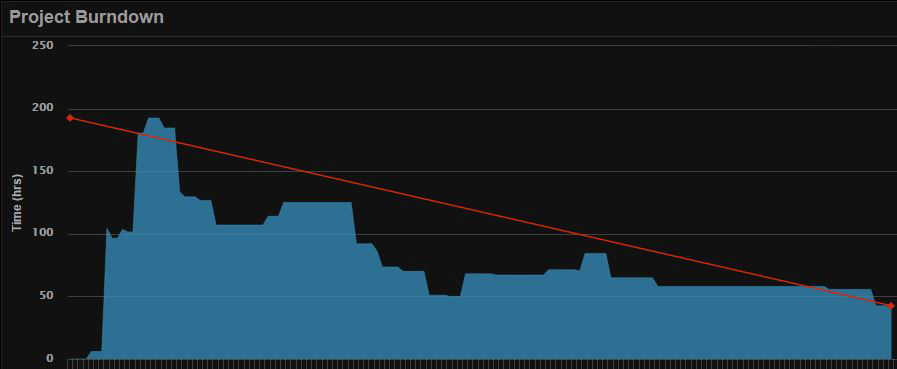
\includegraphics[width=1.0\linewidth]{./appendixImages/AxosoftScreenShot01}
	\textit{Axosoft} Burn-down Chart 
\subsection{}
	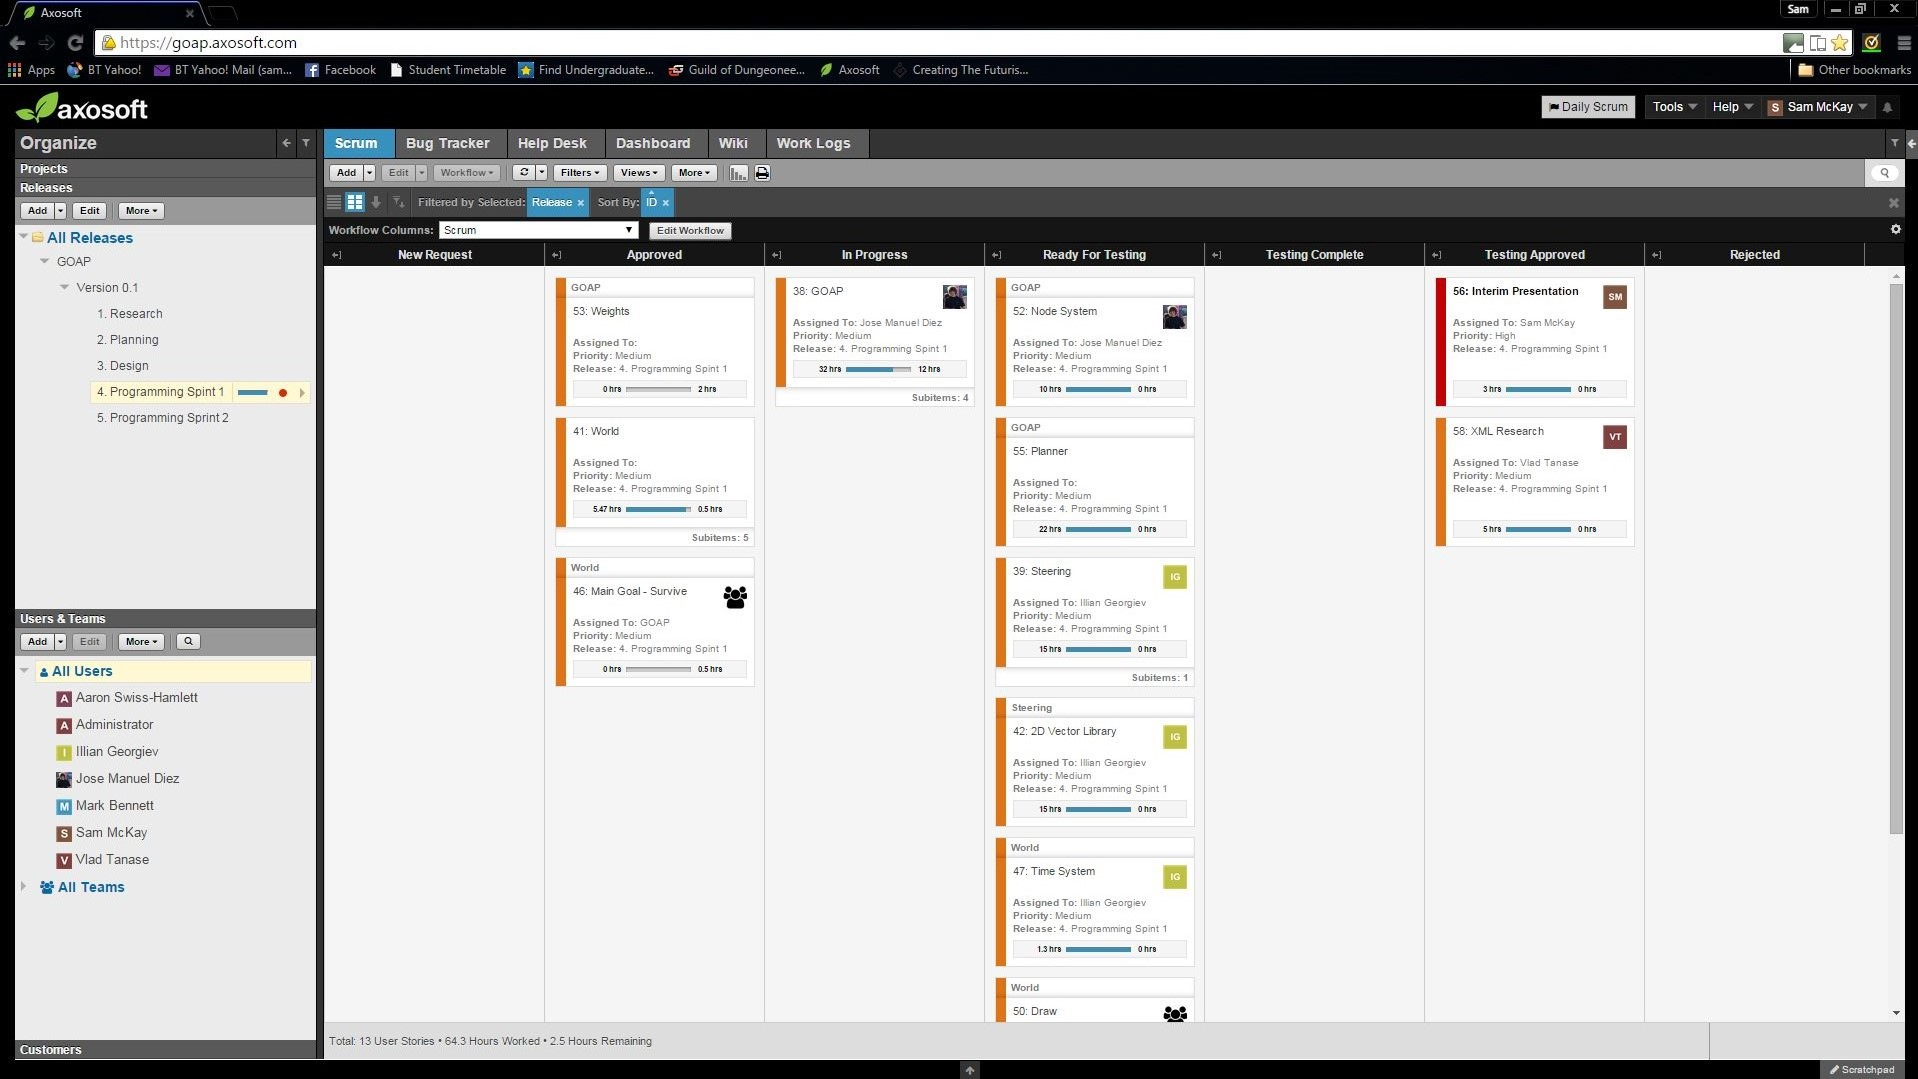
\includegraphics[width=1.0\linewidth]{./appendixImages/AxosoftScreenShot02}
	\textit{Axosoft} User Stories
\pagebreak
\section{}
\pagebreak
\section{}
\pagebreak
\section{}
\pagebreak
\section{}

\end{document}